\documentclass[a4paper,11pt]{article}
\input{/home/tof/Documents/Cozy/latex-include/preambule_lua.tex}
\newcommand{\showprof}{show them}  % comment this line if you don't want to see todo environment
\fancyhead[L]{Algorithme de traitement des images}
\newdate{madate}{10}{09}{2020}
%\fancyhead[R]{\displaydate{madate}} %\today
\fancyhead[R]{Seconde - SNT}
%\fancyhead[R]{Première - NSI}
%\fancyhead[R]{Terminale - NSI}
\fancyfoot[L]{~\\Christophe Viroulaud}
\AtEndDocument{\label{lastpage}}
\fancyfoot[C]{\textbf{Page \thepage/\pageref{lastpage}}}
\fancyfoot[R]{\includegraphics[width=2cm,align=t]{/home/tof/Documents/Cozy/latex-include/cc.png}}
\usepackage{tikz}

\begin{document}
\begin{Form}
\begin{commentprof}
\textbf{traitement-image.zip} sur site
\end{commentprof}
\section{Problématique}
\begin{center}
\begin{tabular}{cc}
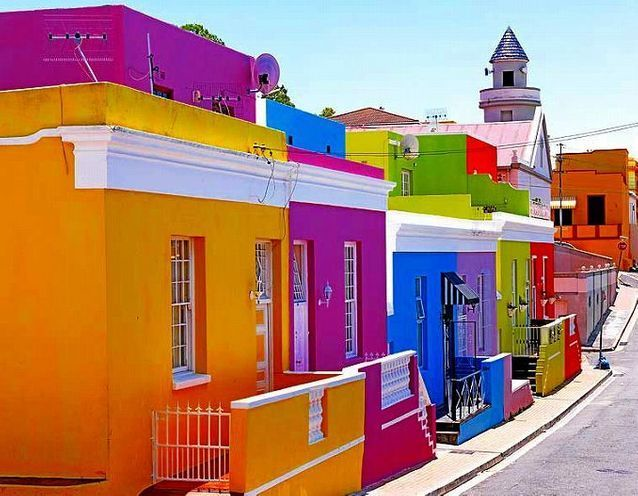
\includegraphics[width=3cm]{ressources/maisons-colorees.png}
 & 
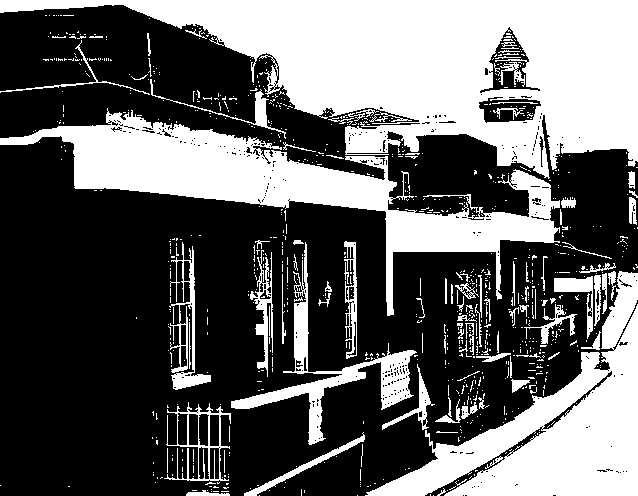
\includegraphics[width=3cm]{ressources/maisons-colorees-NB.png}
 \\ 
\end{tabular} 
\end{center}
À l'aide des notions de langage de programmation, il est possible de construire n'importe quel programme. Mais un programmeur procède par étape.
\begin{center}
\shadowbox{\parbox{10cm}{\centering Comment construire un programme informatique?}}
\end{center}
\section{Déterminer les étapes: l'algorithme}
Pour faire exécuter une tâche à la machine, il faut lui détailler toutes les étapes à réaliser. 
\subsection{Découper en étapes simples}
Pour modifier l'image  il faut effectuer les tâches suivantes:
\begin{itemize}
\item \textbf{Première étape:} stocker l'image en mémoire.
\item \textbf{Deuxième étape:} Modifier chaque pixel.
\item \textbf{Troisième étape:} Enregistrer la nouvelle image.
\end{itemize}
\subsection{Détailler les étapes critiques}
Une image est une grille composée de pixels. Pour transformer l'image couleur, en noir et blanc, il faut effectuer une opération sur chaque pixel.
\begin{center}
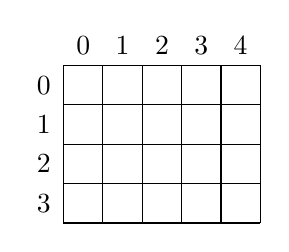
\begin{tikzpicture}[scale=0.5]
\draw (0,0) grid (5,4);

\draw (-0.5,3.5) node{0};
\draw (-0.5,2.5) node{1};
\draw (-0.5,1.5) node{2};
\draw (-0.5,0.5) node{3};
\draw (0.5,4.5) node{0};
\draw (1.5,4.5) node{1};
\draw (2.5,4.5) node{2};
\draw (3.5,4.5) node{3};
\draw (4.5,4.5) node{4};
\end{tikzpicture}
\captionof{figure}{Coordonnées d'un pixel}
\label{matrice}
\end{center}

\textbf{Deuxième étape:} Modifier chaque pixel.
\begin{itemize}
\item Parcourir la grille ligne par ligne.
\begin{itemize}
\item Parcourir la ligne colonne par colonne.
\begin{itemize}
\item Récupérer les couleurs du pixel.
\item Le transformer en noir et blanc.
\end{itemize}
\end{itemize}
\end{itemize}
\section{Coder l'algorithme: le programme}
Il faut ensuite traduire l'algorithme dans le langage de programmation désiré.
\begin{activite}
\begin{enumerate}
\item Télécharger le fichier \emph{traitement-image.zip} sur le site \url{https://cviroulaud.github.io} .
\item Extraire le dossier traitement-image.
\item Ouvrir le logiciel \emph{Spyder}.
\item Depuis le logiciel ouvrir le fichier \emph{noir-blanc.py} .
\item Observer le programme et repérer les trois étapes de l'algorithme.
\item Comment fait-on le choix de transformer le pixel en noir ou blanc?
\item Exécuter le programme.
\item Modifier le programme pour que l'image obtenue soit plus sombre. Recommencer pour qu'elle soit plus claire.
\end{enumerate}
\end{activite}
\section{Créer d'autres algorithmes}
À partir de l'algorithme de base, nous pouvons imaginer d'autres traitements pour la photographie.
\begin{activite}
\begin{enumerate}
\item Dans les cours précédents, retrouver comment obtenir la couleur grise.
\item Enregistrer le programme précédent sous le nom \emph{niveaux-gris.py} .
\item Modifier le programme pour que l'image obtenue soit en nuances de gris.
\item Enregistrer le programme précédent sous le nom \emph{niveaux-rouge.py} .
\item Modifier le programme pour que l'image obtenue ne contienne que les composantes rouges de chaque pixel.
\end{enumerate}
\end{activite}
\end{Form}
\end{document}